%-------------------------------------------------------------------------------
% File: performance.tex
%       
%
% Author: Marco Pinna
%         Created on 14/06/2022
%-------------------------------------------------------------------------------
\chapter{Performance}\label{ch:performance}
This final chapter concerns the performance evaluation of the different implementations of the algorithms.\\
Deployment and testing were all performed on a cluster of four virtual machines provided by the University. Each of them was a Ubuntu machine with 2 cores and 8 GB of RAM.\\
The Key Performance Indexes (KPIs) that were studied were:
\begin{itemize}
	\item the \colorbox{gray!30}{\large \texttt{Map output bytes}}, i.e. the number of bytes output by the Mappers to be sent to the reducers. This impacts the amount of traffic to be sent over the network during the execution of the algorithm.
	\item the \colorbox{gray!30}{\large \texttt{wall time}}, i.e. the total time elapsed between the launch of the program and the its completion, with the output written to HDFS
\end{itemize}

The tests were performed with different configurations, obtained by changing the following paremters:\\
\begin{itemize}
	\item the FPR \colorbox{gray!30}{\large \texttt{p}} (v. \ref{sec:bloom_filters}): its value ranges from 0.00001 (0.001 \%) to 0.1 (10 \%), incrementing each time by an order of magnitude
	\item the number of hashing functions \colorbox{gray!30}{\large \texttt{k}}: its values range from 3 to 9, with increments of 2. Furthermore, configurations with no constraints on the value of \texttt{k} were tested.
	\item the number of mappers: its value ranges from 4 to 12 with increments of 2
\end{itemize}

Each test was run 10 times to limit the impact of outliers.% This yielded a total of TODO tests.

\section{Hadoop map output bytes}

\subsection*{Map output bytes as function of \textit{p}}

Figure \ref{fig:MapOutputBytesP} shows the amount of bytes sent by the mappers to the reducers, as function of the FPR \texttt{p}, for both implementations and two different values of \textit{k}.\\

\begin{figure}[H]
    \begin{center}
        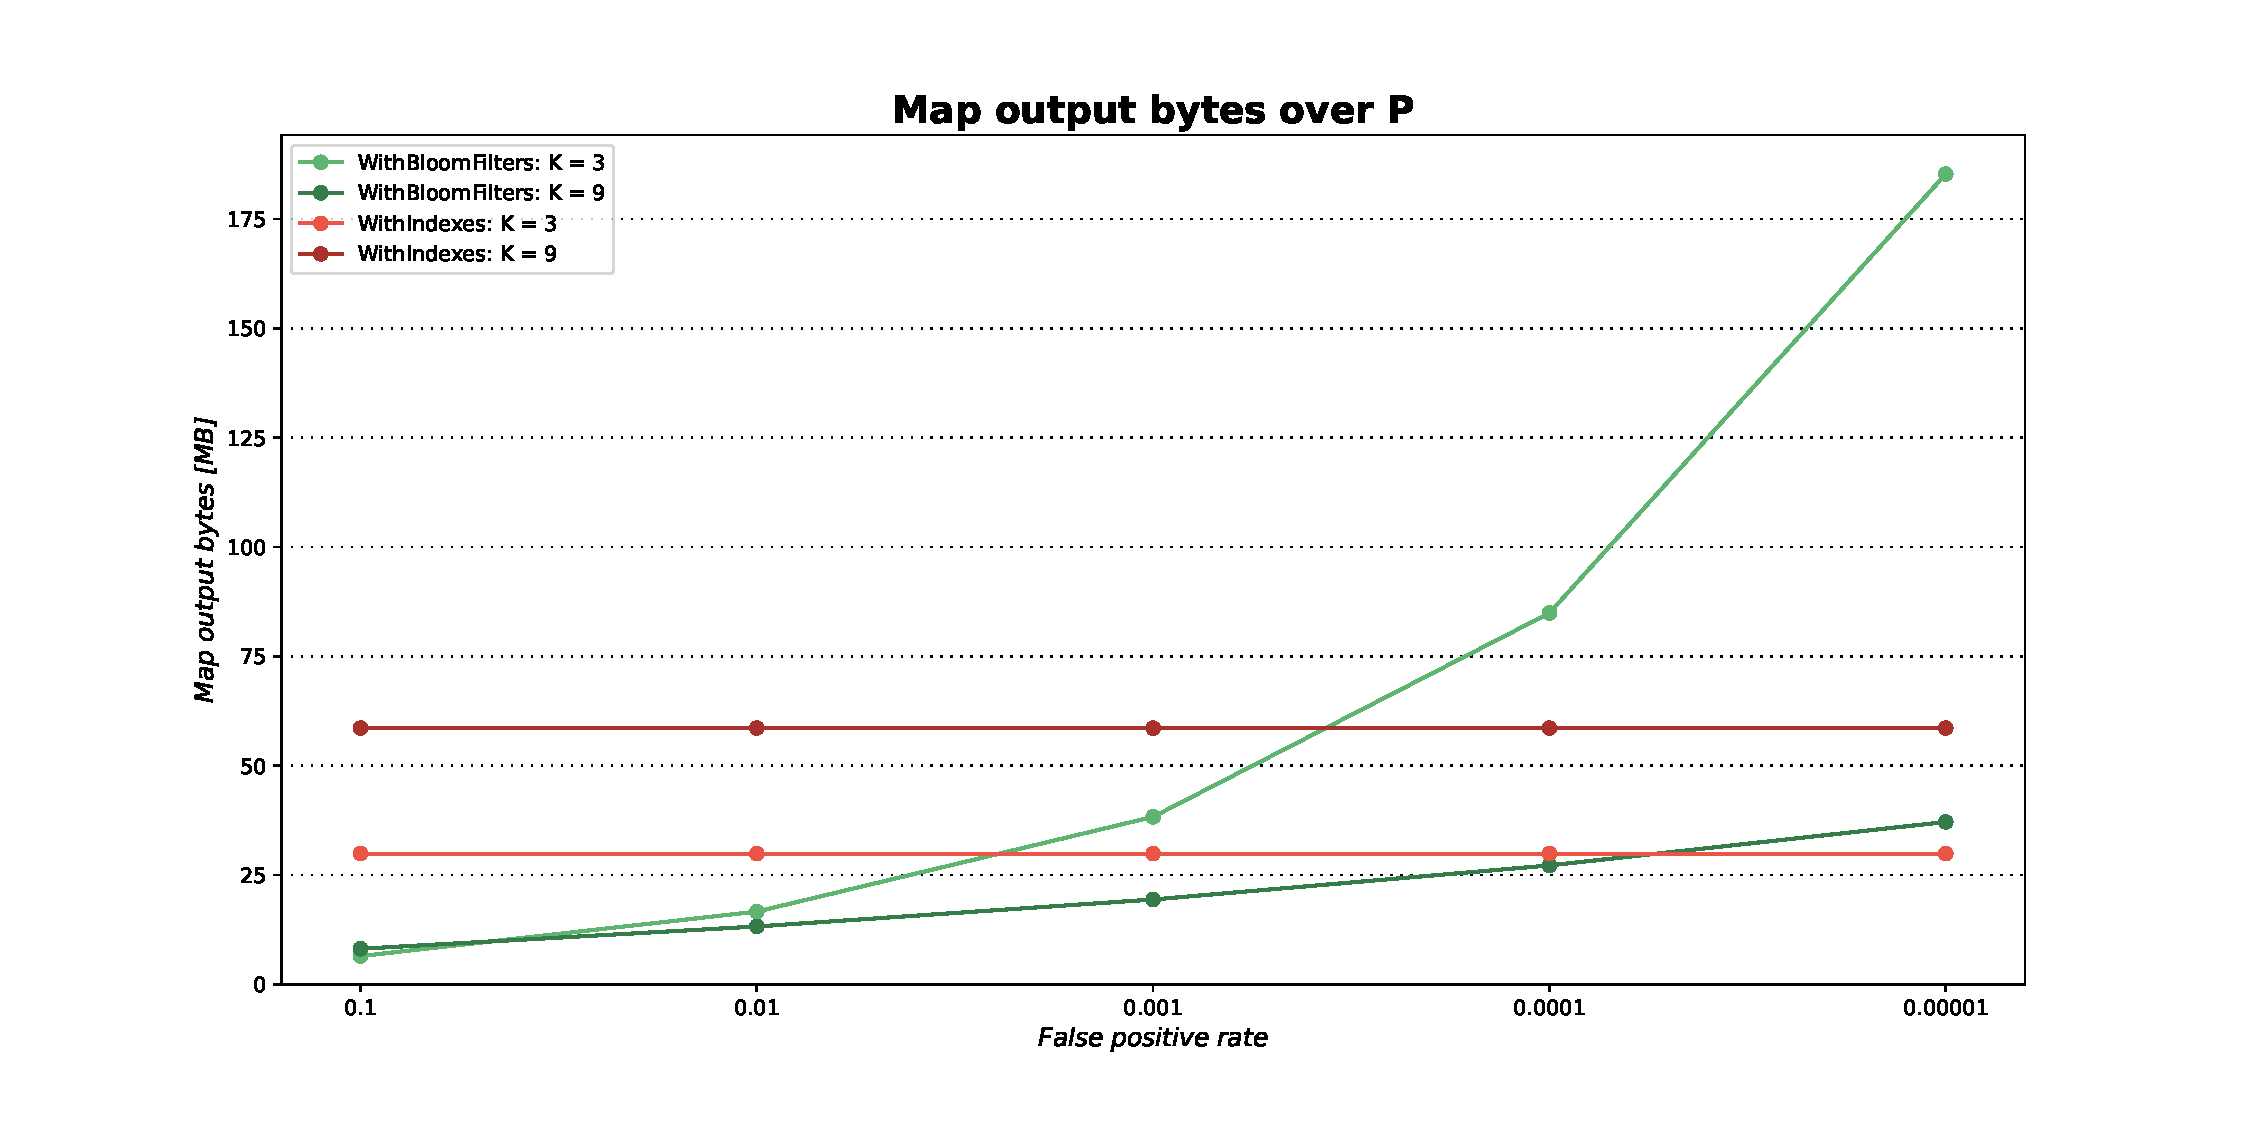
\includegraphics[scale=.45,trim={3cm 0 3cm 0},clip]{img/MapOutputBytesP.pdf}
    \end{center}
    \vspace*{-0.5cm}
    \caption{Map output bytes as function of \texttt{p}}
    \label{fig:MapOutputBytesP}
\end{figure}

\noindent As it stands out from the red lines, the amount of bytes produced by the mappers in the \textit{withIndexes} implementation does not depend on \textit{p}, but it only increases with \texttt{k}. This makes complete sense since, regardless of the size \texttt{m} of the Bloom filter, the number of indexes is always equal to \texttt{k}. Although the two values of \texttt{k} considered in the plot have a ratio of 3, the same ratio is not preserved in the values of the red line: this is probably due to some overhead bytes added by the serialization process of the objects and network communication.\\
On the other hand, in the \textit{withBloomFilters} implementation, the amount of bytes sent by the mappers increases as \texttt{p} decreases, as it can be seen especially for lower values of \texttt{k} (light green plot in the figure).

\subsection*{Map output bytes as function of \textit{p} with optimal \textit{k}}

Figure \ref{fig:MapOutputBytesP_bestK} shows the amount of bytes sent by the mappers to the reducers, as function of the FPR \texttt{p}, for both implementations and an the optimal value for \texttt{k}.\\

\begin{figure}[H]
    \begin{center}
        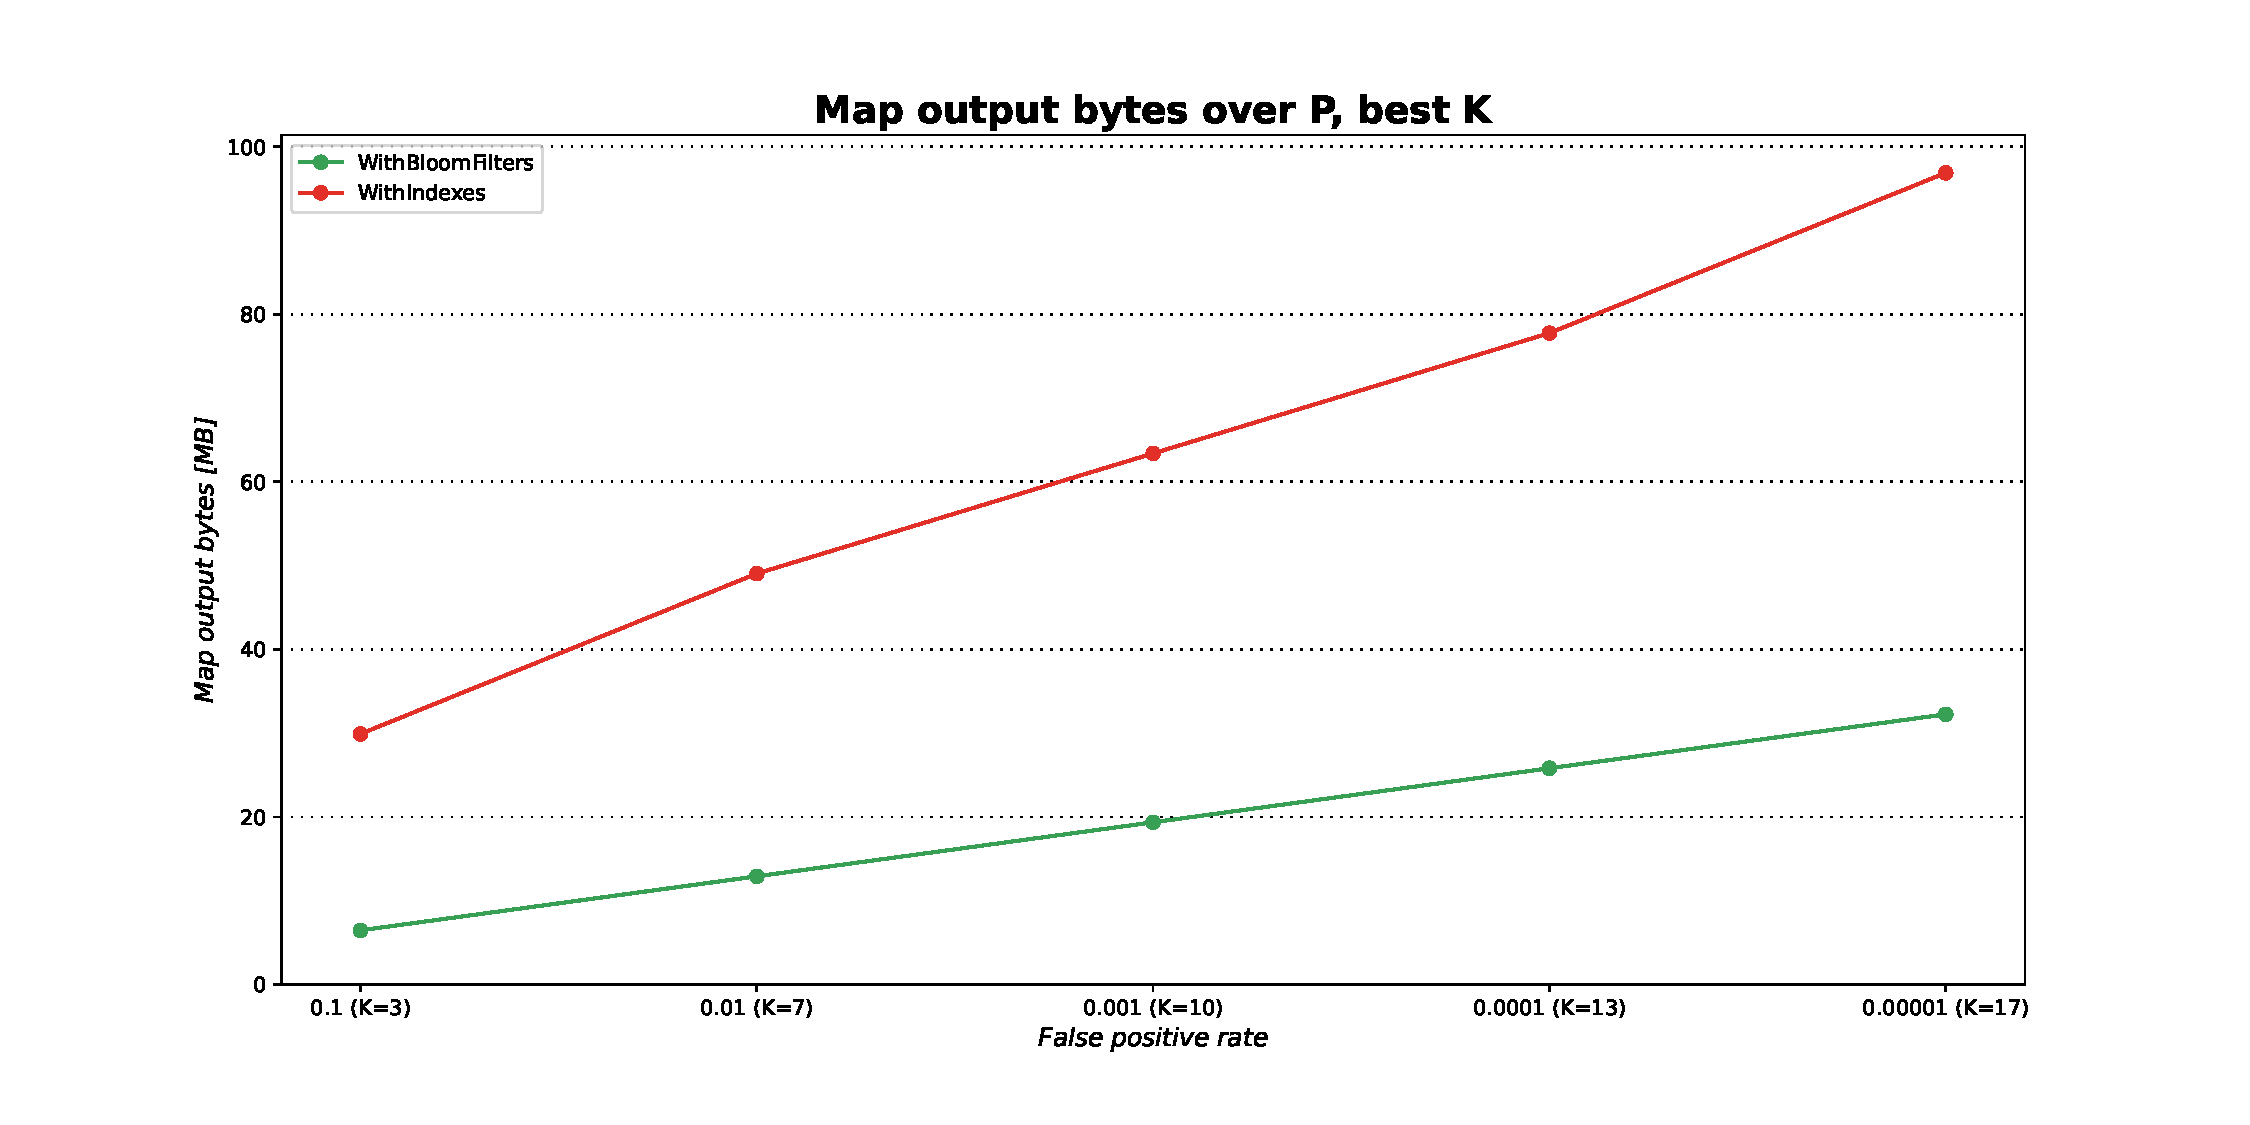
\includegraphics[scale=.45,trim={3cm 0 3cm 0},clip]{img/MapOutputBytesP_bestK.pdf}
    \end{center}
    \vspace*{-0.5cm}
    \caption{Map output bytes as function of \texttt{p} with optimal value of \texttt{k}}
    \label{fig:MapOutputBytesP_bestK}
\end{figure}


\noindent Both plots seem to follow a linear trend, which is consistent with the first and second formulas in \ref{eq:parameters}: a geometric progression of \texttt{p} yields an arithmetic progression (because of the logarithm in the first expression) in the value of \texttt{m}. The optimal value of \texttt{k} is in turn linearly dependent on \texttt{m}.\\
These two relations explain, respectively, the linear increase in the size of bloom filters and the linear increase in the amount of indexes to be sent.

\subsection*{Map output bytes as function of the number of mappers}

Figure \ref{fig:MapOutputBytesMappers} shows the amount of bytes sent by the mappers to the reducers, as function of the number of mappers with optimal values of \texttt{k}, for both implementations.\\

\begin{figure}[H]
    \begin{center}
        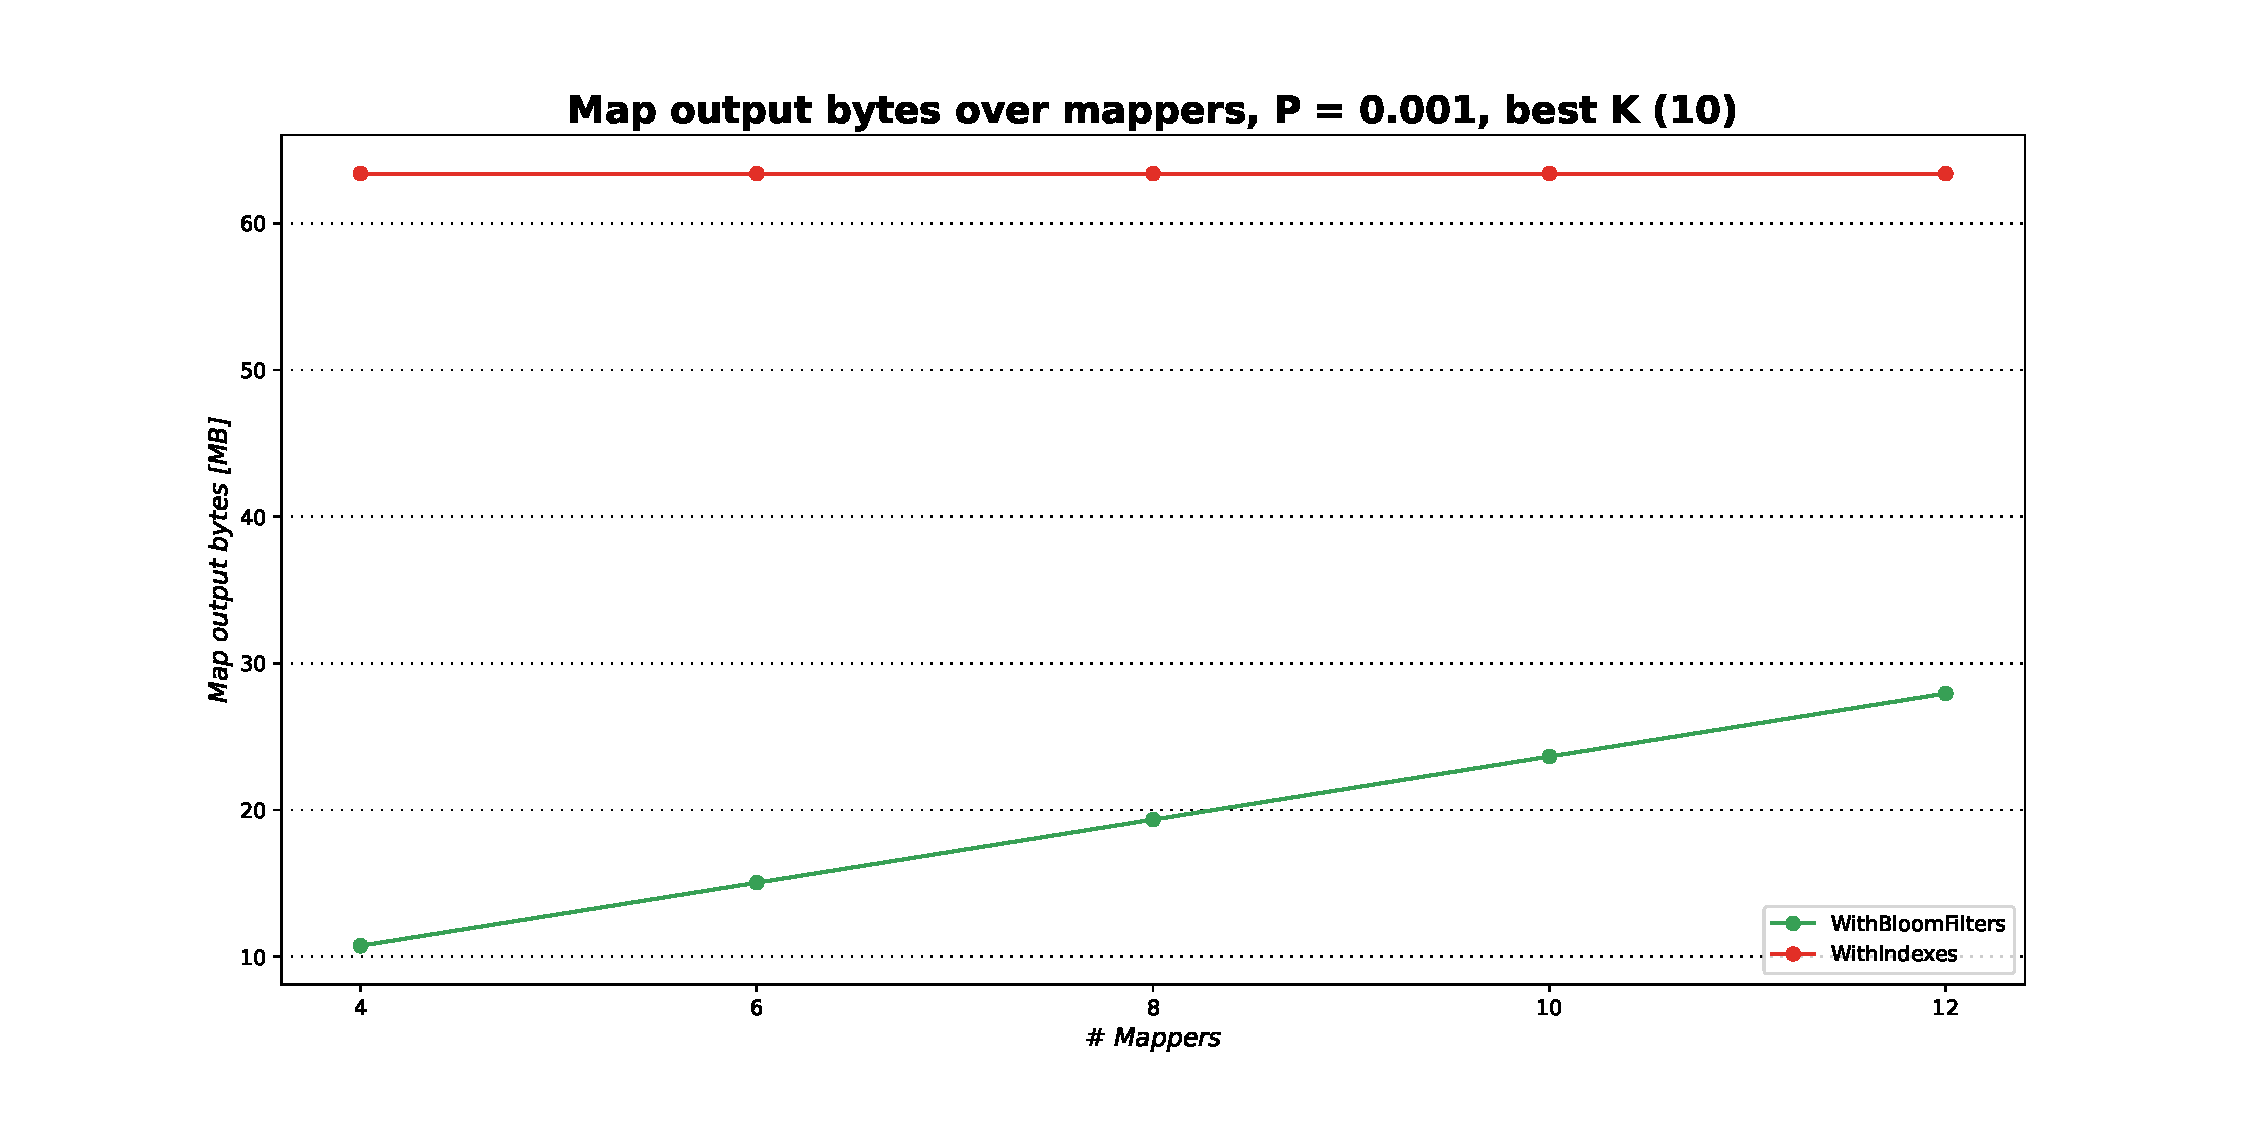
\includegraphics[scale=.45,trim={3cm 0 3cm 0},clip]{img/MapOutputBytesMappers.pdf}
    \end{center}
    \vspace*{-0.5cm}
    \caption{Map output bytes as function of the number of mappers}
    \label{fig:MapOutputBytesMappers}
\end{figure}

\noindent The explanation of this plot is quite trivial: in the \textit{withBloomFilters} implementation every mapper has to create 10 Bloom filters and send them, regardless of how ``full" they will be. Therefore, the overall amount of bytes sent by all the mappers to the reducer(s) will increase linearly with an increase in the number of mappers.\\
On the other hand, the \textit{withIndexes} implementation always has a constant amount of traffic for fixes values of \texttt{p} and \texttt{k}, regardless of the number of mappers: this is because the total amount of indexes that are sent by all the mappers only depends on the size of the dataset. A bigger number of mappers will imply smaller partitions with fewer indexes being sent by each mapper; their overall amount will however be the same when they are received by the reducer(s).

\section{Hadoop wall time}

\subsection*{Wall time as function of \textit{p} with optimal \textit{k}}

Figure \ref{fig:hadoop_wallTimeP_bestK} shows the amount take taken by the MapReduce algorithm to run from start to finish as function of \texttt{p}, with an optimal value for \texttt{k}, for both implementations.\\

\begin{figure}[H]
    \begin{center}
        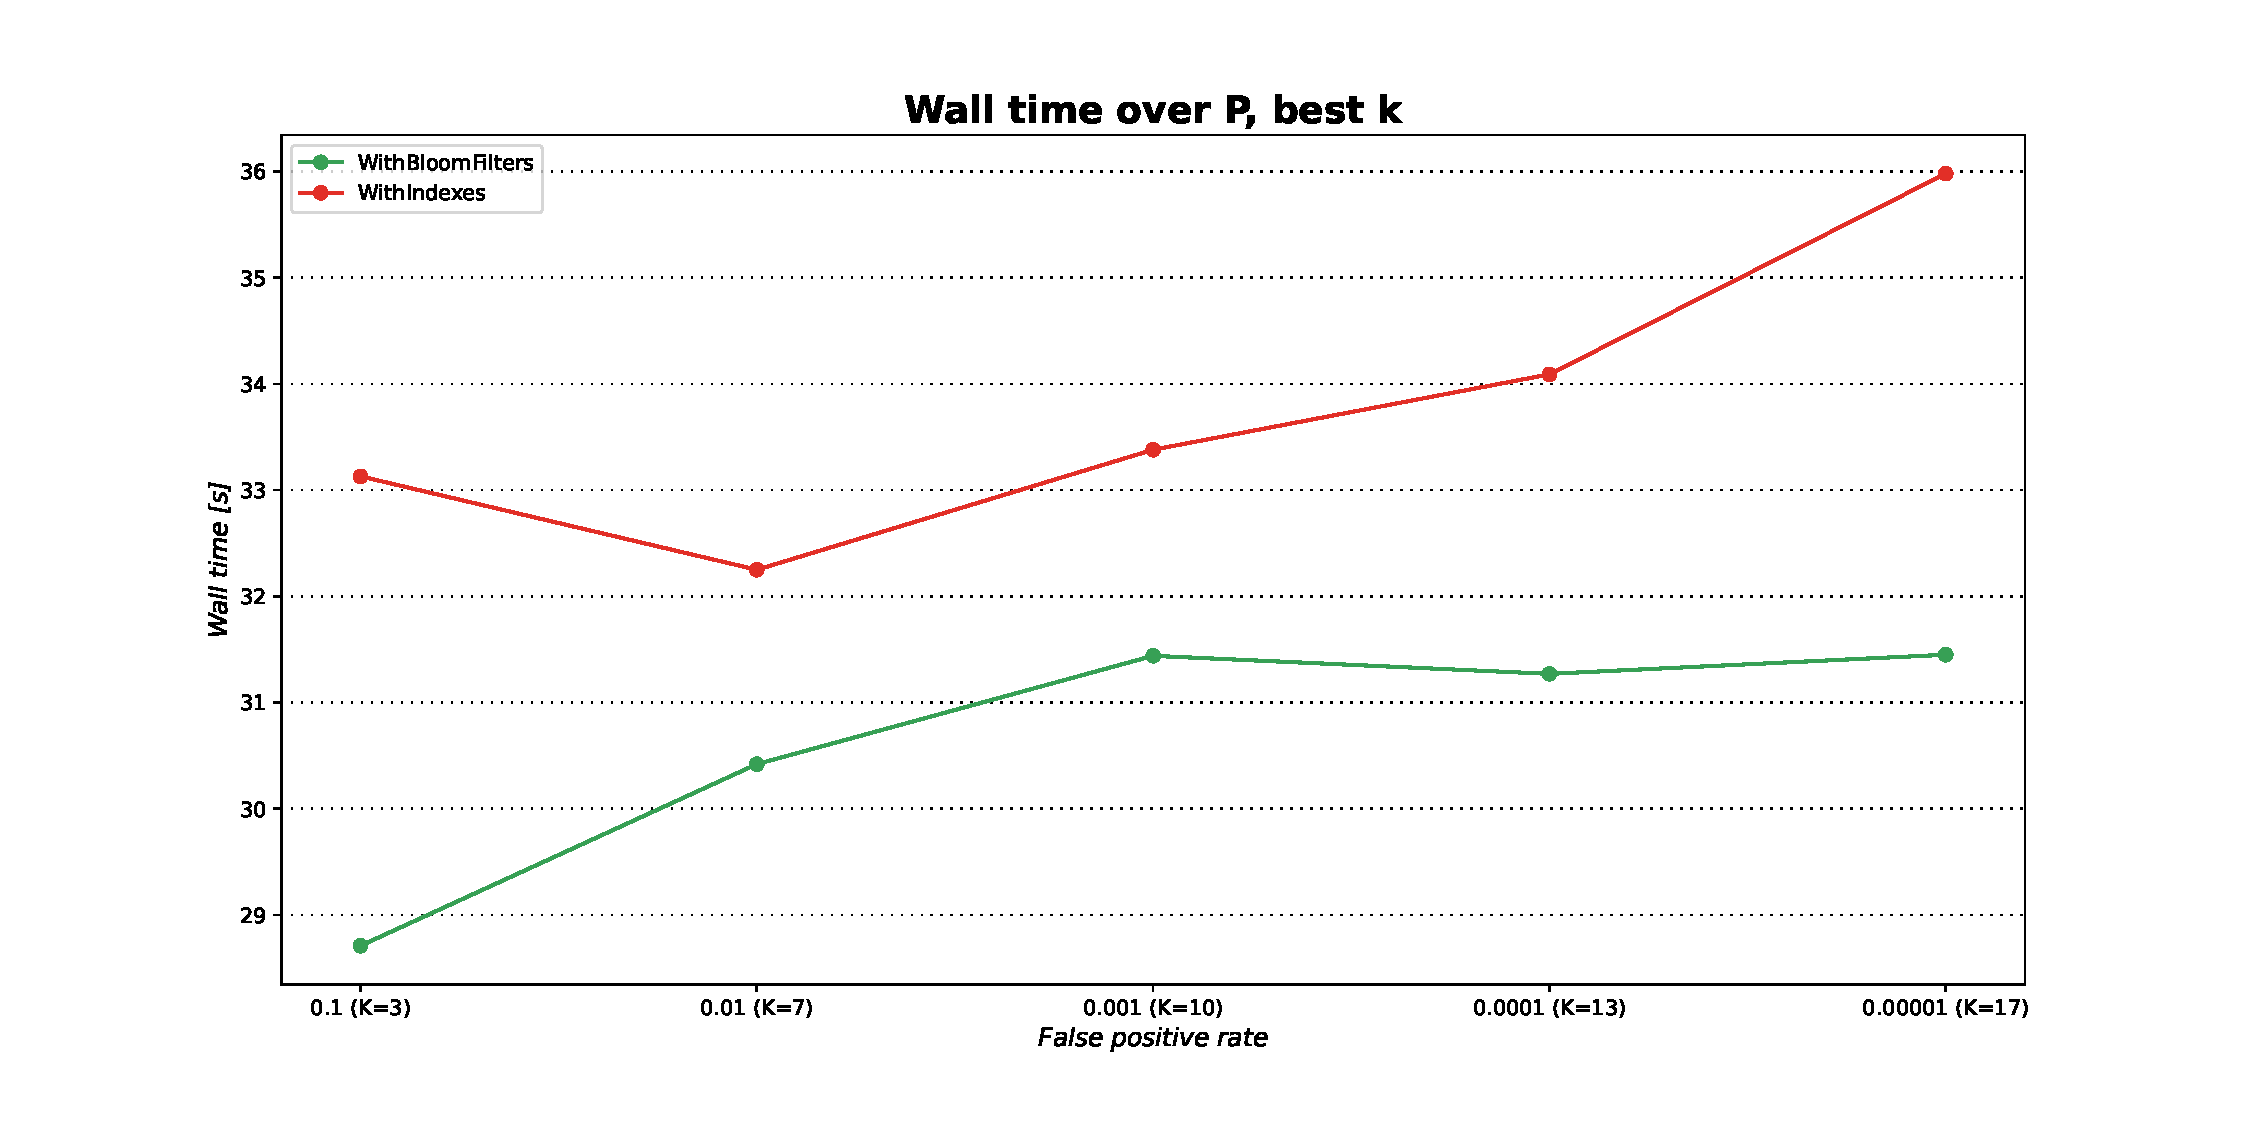
\includegraphics[scale=.45,trim={3cm 0 3cm 0},clip]{img/hadoop_wallTimeP_bestK.pdf}
    \end{center}
    \vspace*{-0.5cm}
    \caption{Wall time as function of \texttt{p} with optimal values for \texttt{k}}
    \label{fig:hadoop_wallTimeP_bestK}
\end{figure}

\noindent The plots are quite instable and noisy, which is likely caused by the fact that the cluster on which the tests were run was not a very stable and controlled environment and because of the low amount of replications of the tests.\\
Nevertheless it seems clear that the \textit{withBloomFilters} implementation proves to be more efficient, time-wise, regardless of the value of the FPR.

\subsection*{Wall time as function of the number of mappers, fixed \textit{p} and optimal \textit{k}}

Figure \ref{fig:hadoop_wallTimeMap} shows the amount take taken by the MapReduce algorithm to run from start to finish as function of the number of mappers, with a fixed value of \texttt{p} and an optimal value for \texttt{k}, for both implementations.\\

\begin{figure}[H]
    \begin{center}
        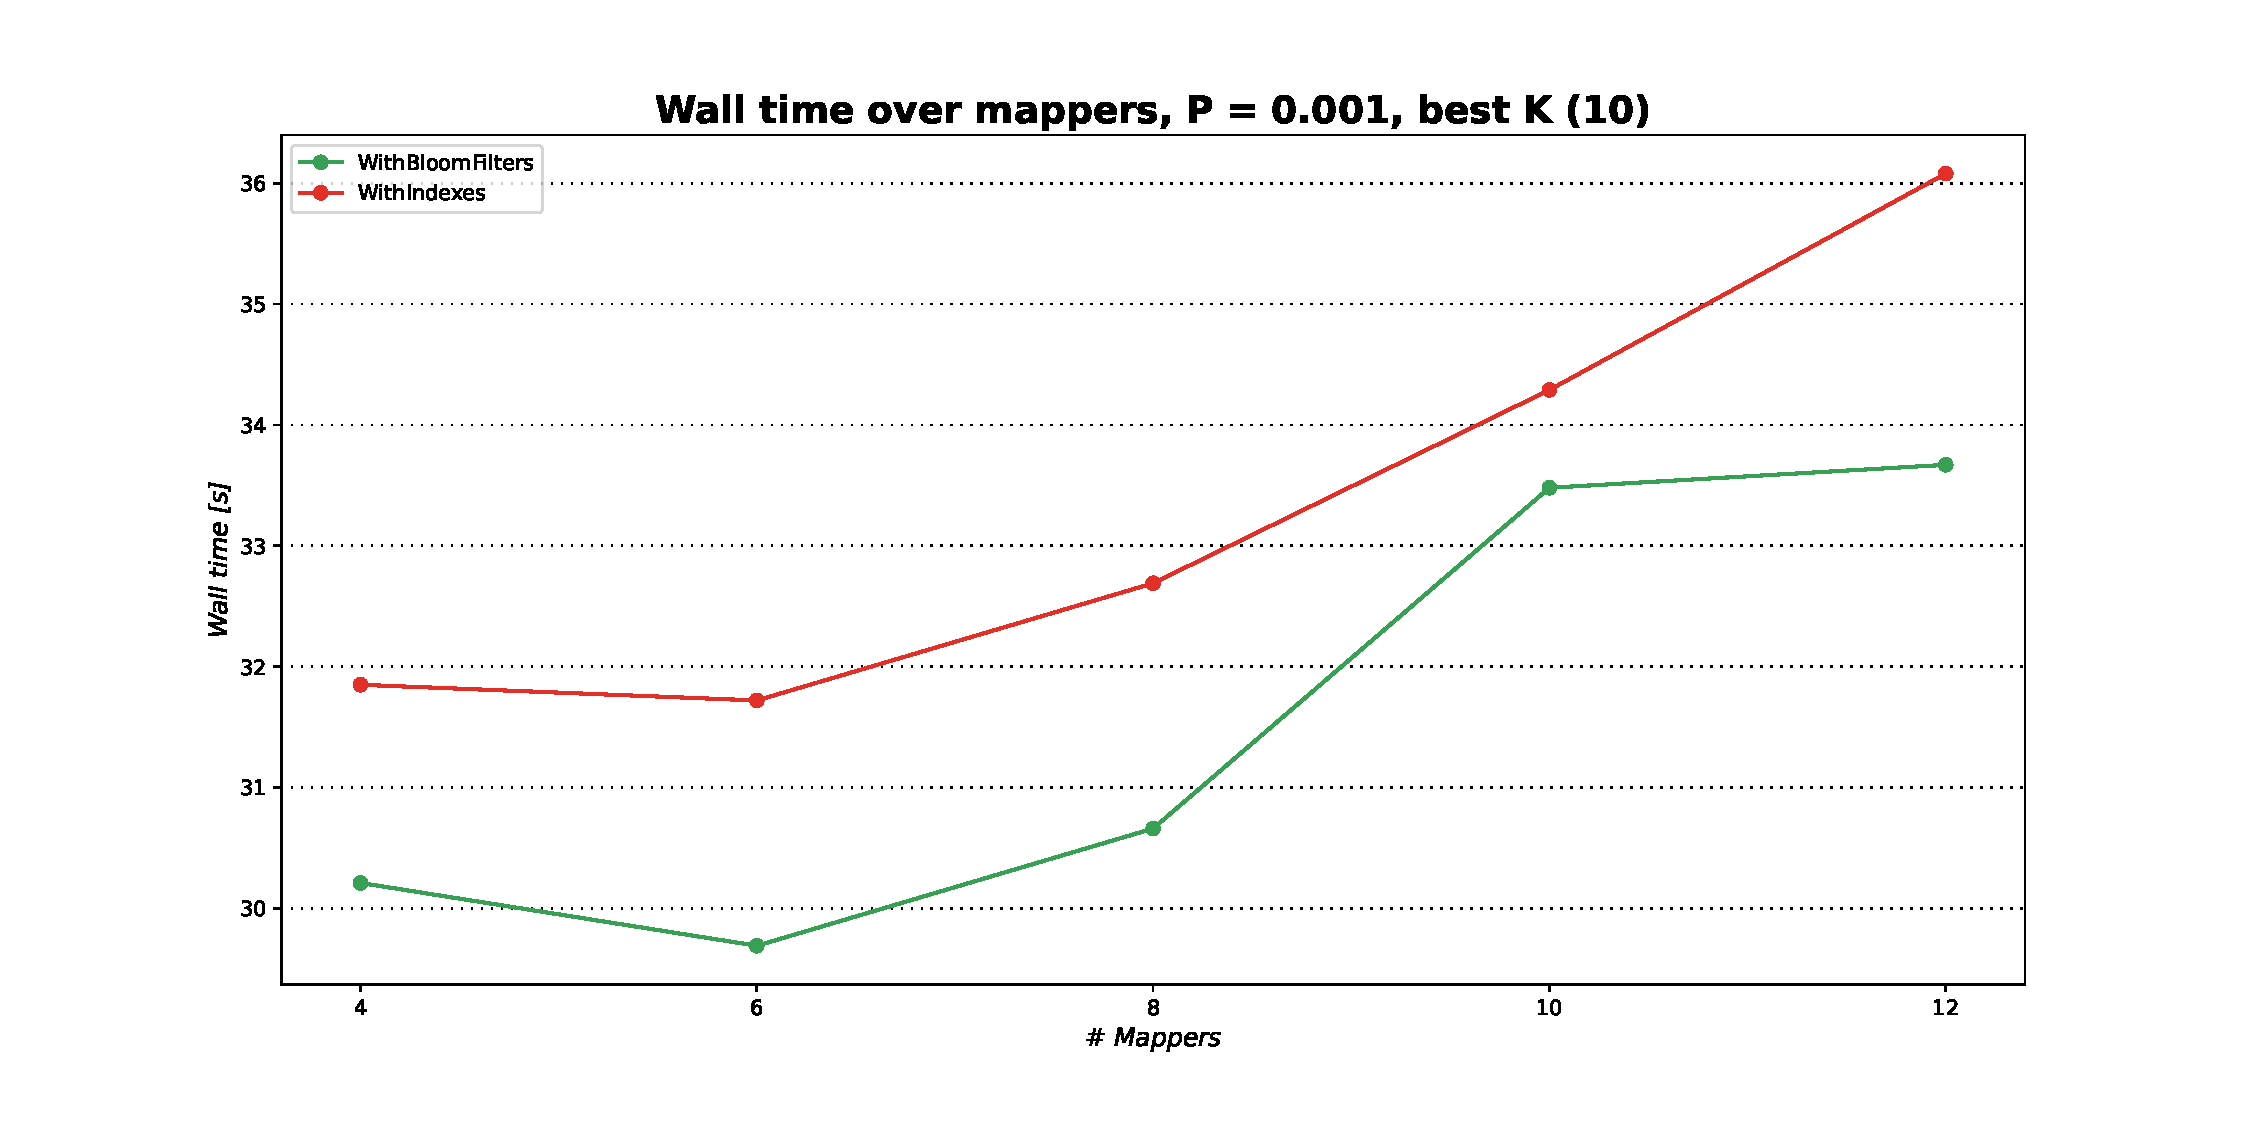
\includegraphics[scale=.45,trim={3cm 0 3cm 0},clip]{img/hadoop_wallTimeMap.pdf}
    \end{center}
    \vspace*{-0.5cm}
    \caption{Wall time as function of the number of mappers}
    \label{fig:hadoop_wallTimeMap}
\end{figure}

\noindent Both plots show a minimum for a number of mappers equal to 6. As mentioned in chapter \ref{ch:hadoop}, the best practice suggests to assign from 1 to 1.5 cores to each mapper. The two minima in 6 correspond to 1.33 cores assigned to each mapper, which proves the best-practice to be well-founded.

\section{Hadoop vs Spark}

In this final section a brief comparison of the two implementations both in Hadoop and in Spark is presented.

\subsection*{Wall time as function of \textit{p} with optimal \textit{k}}

Figure \ref{fig:hadoopSpark_wallTimeP_bestK} shows the amount take taken by the MapReduce algorithm to run from start to finish, as function of \texttt{p}, with optimal values of \texttt{k}, for both implementations and both frameworks.\\

\begin{figure}[H]
    \begin{center}
        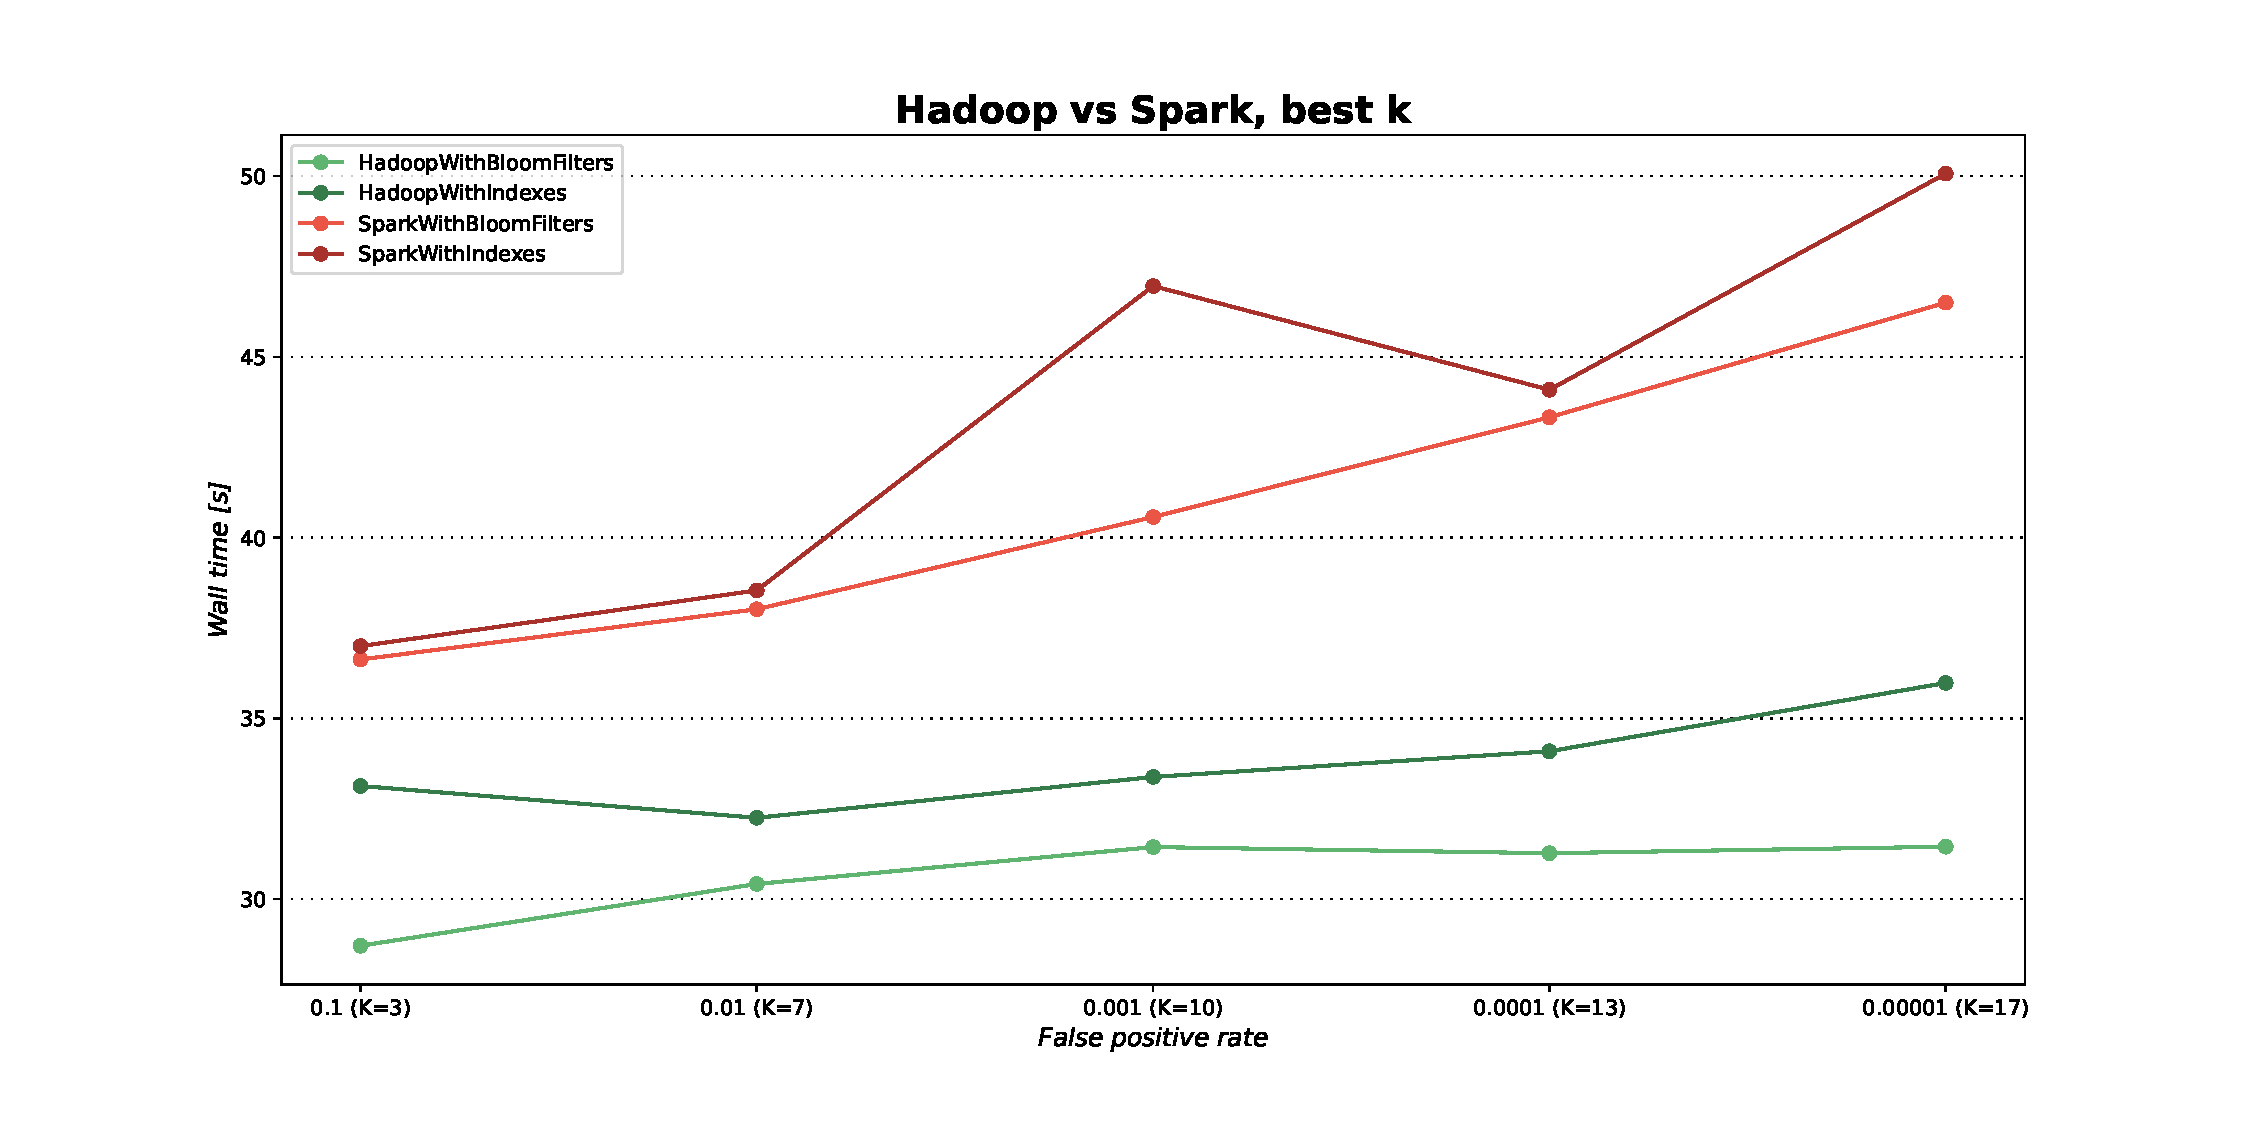
\includegraphics[scale=.45,trim={3cm 0 3cm 0},clip]{img/hadoopSpark_wallTimeP_bestK.pdf}
    \end{center}
    \vspace*{-0.5cm}
    \caption{Wall time as function of \texttt{p} with optimal values for \texttt{k}, Hadoop vs Spark}
    \label{fig:hadoopSpark_wallTimeP_bestK}
\end{figure}

\noindent Contrarily  to what it was expected, Hadoop is faster than Spark on both implementations, despite using intermediate data writes on disks, as opposed to Spark which uses RAM.\\
This apparently abnormal behaviour was thought to be caused by the nature of the algorithm, which does not really take advantage of the efficiency of Spark on multi-passes.